\begin{frame}
\frametitle{Кеширующий алокатор}
\begin{itemize}
  \item Мы умеем алоцировать большие блоки памяти
  \begin{itemize}
    \item мы можем алоцировать большие блоки и разделять их на меньшие блоки
    фиксированного размера;
    \item работать с блоками фиксированного размера проще.
  \end{itemize}
  \item Для объектов одного типа можно сэкономить на инициализации:
  \begin{itemize}
    \item некоторые поля объектов при освобождении находятся в "исходном"
    состоянии;
    \item например, mutex/lock должен быть отпущен перед освобождением памяти, а
    счетчик ссылок скорее всего равен 0/1;
    \item инициализировать такие поля при повторной алокации не нужно;
    \item \href{https://www.usenix.org/legacy/publications/library/proceedings/bos94/full_papers/bonwick.a}{Jeff Bonwik, The Slab Allocator: An Object-Caching
    Kernel Memory Allocator}.
  \end{itemize}
\end{itemize}
\end{frame}

\begin{frame}
\frametitle{Slab Allocator}
\begin{itemize}
  \item Базовым понятие Slab Allocator-а является Slab:
  \begin{itemize}
    \item Slab - пул/кеш объектов/регионов (далее просто объекты) памяти
    фиксированного размера;
    \item Slab - большое регион памяти, который мы разделяем на меньшие кусочик,
    а также управляющие структуры необходимые для алокации;
  \end{itemize}
  \item Для каждого объекта Slab-а есть дескриптор:
  \begin{itemize}
    \item дескрипторы свободных объектов связаны в список;
    \item все объекты одного размера, при алокации мы можем взять любой из них.
  \end{itemize}
\end{itemize}
\end{frame}

\begin{frame}
\frametitle{Slab для маленьких объектов}
\begin{center}
  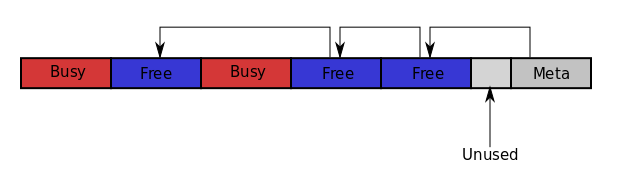
\includegraphics[width=0.8\textwidth]{slab_small.png}
\end{center}
\begin{itemize}
  \item Для маленьких объектов сами объекты и управляющие структуры можно
  хранить вместе:
  \begin{itemize}
    \item пока объект свободен мы можем его использовать как дескриптор;
    \item занятые объекты мы никак не отслеживаем.
  \end{itemize}
  \item Какие объекты считать маленькими?
  \begin{itemize}
    \item в оригианльной статье объекты меньше $1/8 \times PAGE\_SIZE$. 
  \end{itemize}
\end{itemize}
\end{frame}

\begin{frame}
\frametitle{Slab для больших объектов}
\begin{center}
  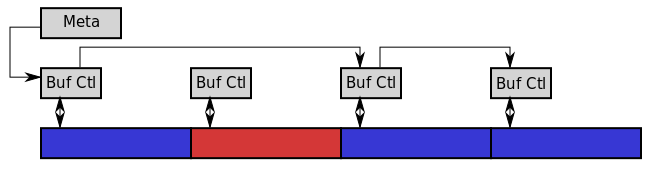
\includegraphics[width=0.8\textwidth]{slab_large.png}
\end{center}
\begin{itemize}
  \item Для больших объектов управляющие структуры алоцируются отдельно:
  \begin{itemize}
    \item мы можем алоцировать их как маленькие объекты;
    \item нам нужно знать был ли объект уже инициализирован или нет;
    \item если вы не оптимизируете инициализацию - вам это не нужно.
  \end{itemize}
\end{itemize}
\end{frame}
